\section{Mengen und Funktionen}

\begin{frame}
  {Was ist eine Menge?}
  \onslide<+->
  \onslide<+->
  Eine \alert{frei definierbare ungeordnete Sammlung von diskreten Objekten}\\
  \begin{itemize}[<+->]
    \item Zahlen
    \item Menschen
    \item Schuhe
    \item Wörter
    \item \ldots
      \Halbzeile
    \item nicht unbedingt zweckgebunden
    \item \orongsch{jedes Objekt maximal einmal in jeder Menge}
  \end{itemize}
  \centering
  \Zeile
  \onslide<+->
  Das Wesentliche von heute in \citet[Kapitel~1--4]{ParteeEa1990}
\end{frame}

\begin{frame}
  {Notation und Beispiele für Mengen}
  \onslide<+->
  \onslide<+->
  Mengendefinition \alert{$\{\}$}, Elementstatus $\in$\\
  \Zeile
  \begin{itemize}[<+->]
    \item M\Sub{1} = \alert{$\{a,b,c\}$} (Menge von Buchstaben)
      \Halbzeile
    \item N\Sub{1} = \alert{$\{$\textit{`my book'}$\}$} (einelementige Menge, enthält eine NP)
      \begin{itemize}[<+->]
        \item vs. \alert{N\Sub{2} = $\{$\textit{my book}$\}$} (einelementige Menge, enthält mein Buch)
        \item vs. \alert{N\Sub{3} = $\{$\textit{`my', `book'}$\}$} (Menge von Wörtern)
      \end{itemize}
      \Halbzeile
    \item auch möglich: \orongsch{N\Sub{4} = $\{$\textit{`my', book}$\}$}
      \Halbzeile
    \item definiert über eine Eigenschaft der Elemente (zwei Notationen):\\
      M\Sub{2} = \gruen{$\{$\textit{x: x is one of the first three letters of the alphabet}$\}$}\\
      M\Sub{2} = \gruen{$\{x$|\textit{x is one of the first three letters of the alphabet}$\}$}
      \Halbzeile
    \item \alert{U}: die universelle Menge (alle Objekte)
  \end{itemize}
\end{frame}

\begin{frame}
  {Identität von Mengen}
  \onslide<+->
  \onslide<+->
  Zwei Mengen mit exakt den gleichen Elementen sind \alert{identisch}.\\
  \Zeile 
  \begin{itemize}[<+->]
    \item \alert{$\{a,b,c\}$} = \gruen{$\{\text{\textit{x:x is one of the first three letters of the alphabet}}\}$}
      \Halbzeile
    \item \alert{$\{\text{\textit{x: x is human}}\}$} = \gruen{$\{\text{\textit{x: x is from the Earth, a primate but not an ape}}\}$}
  \end{itemize}
\end{frame}

\begin{frame}
  {Teilmengen und Obermengen}
  \onslide<+->
  \onslide<+->
  \alert{Teilmenge} | Eine Menge N, die kein Element enthält,\\
  das nicht auch in Menge M enthalten ist (umg.\ \alert{Obermenge}).\\
  \Halbzeile
  \onslide<+->
  Teilmenge oder Identität $\subseteq$\\
  Obermenge oder Identität $\supseteq$\\
  \Zeile
  \begin{itemize}[<+->]
    \item $\{a\}\alert{\subseteq}\{a,b,c\}$ und $\{a,b,c\}\alert{\supseteq}\{a\}$
    \item $\{a\} \alert{\subseteq}\{a,b,c\}$ und $\{a,b,c\}\alert{\supseteq}\{a\}$
    \item $\{a,b,c\}\alert{\subseteq}\{a,b,c\}$
      \Halbzeile
    \item $\{a,b,c,d\}\orongsch{\not\subseteq}\{a,b,c\}$ und $\{a,b,c\}\orongsch{\not\supseteq}\{a,b,c,d\}$
      \Halbzeile
    \item $\{\text{\textit{x: x is human}}\}\gruen{\subseteq}\{\text{\textit{x: is an ape}}\}$
  \end{itemize}
\end{frame}


\begin{frame}
  {Echte Teilmengen und Obermengen}
  \onslide<+->
  \onslide<+->
  \alert{Echte Teilmenge} | Eine Menge N, die kein Element enthält,\\
  das nicht auch in Menge M enthalten ist, und die nicht mit M identisch ist.\\
  \Halbzeile
  \onslide<+->
  Echte Teilmenge $\subset$\\
  Echte Obermenge $\supset$\\
  \Zeile
  \begin{itemize}[<+->]
    \item $\{a\}\gruen{\subset}\{a,b,c\}$ und $\{a\}\alert{\subset}\{a,b,c\}$
    \item $\{a,b,c\}\orongsch{\not\subset}\{a,b,c\}$ aber $\{a,b,c\}\orongsch{\subseteq}\{a,b,c\}$
  \end{itemize}
\end{frame}

\begin{frame}
  {Elemente vs.\ Teilmengen}
  \onslide<+->
  \begin{itemize}[<+->]
    \item Achtung bei Mengen von Mengen
      \Viertelzeile
      \begin{itemize}[<+->]
        \item $\{\{a\}\}\orongsch{\not\subset}\{a,b,c\}$
        \item $\{\{a\}\}\orongsch{\not\subseteq}\{a,b,c\}$
        \item $\{\{a\}\}\orongsch{\not\in}\{a,b,c\}$
      \end{itemize}
    \Zeile
    \item für leere Menge \grau{$\{\}$ oder $\emptyset$}
      \Viertelzeile
      \begin{itemize}[<+->]
        \item $\{\}\alert{\subset}\text{jede anderen Menge}$
        \item $\{\}\orongsch{\not\in}\{\}$
      \end{itemize}
  \end{itemize}
\end{frame}

\begin{frame}
  {Logik mit Mengen, Teilmengen und Elementen}
  \onslide<+->
  \begin{itemize}[<+->]
    \item Logik mit Mengen
        \begin{itemize}[<+->]
        \item \textit{Alle Anglistikprofessoren sind menschlich.}\\
          \textit{Herr Webelhuth ist Anglistikprofessor.}
        \item w = Herr Webelhuth\\
          $E=\{\text{\textit{x: x is a professor of English Linguistics}}\}$\\
          $H=\{\text{\textit{x: x is human}}\}$
        \item Aus \alert{$w\in E$} und \alert{$E\subset H$} folgt \gruen{$w\in H$}
      \end{itemize}
      \Halbzeile
    \item Aber
      \begin{itemize}[<+->]
        \item \textit{Die Anglistikprofessoren sind zahlreich.}
        \item $N=\{\text{\textit{x: x is a set with many members}}\}$
        \item Aus \alert{w $\in$ E} und \orongsch{E $\in$ N} folgt nicht \alert{w $\in$ N}
        \item Vergleiche: \textit{*Herr Webelhuth ist zahlreich.}
      \end{itemize}
  \end{itemize}
\end{frame}

\begin{frame}
  {Potenzmengen (power sets)}
  \label{slide:potenzmenge}
  \onslide<+->
  \onslide<+->
  Potenzmenge $\wp(\cdot)$ | Für jede Menge M: \alert{$\wp(M)=\{X:X\subseteq M\}$}\\
  \Halbzeile
  \begin{itemize}[<+->]
    \item Beispiel
      \begin{itemize}[<+->]
        \item $M=\{\gruen<6,9,10,12>{a},\gruen<7,9,11,12>{b},\gruen<8,10,11,12>{c}\}$
        \item $\wp(M)=\{%
           \only<6->{\gruen<6>{\{a\}}}%
           \only<7->{,\gruen<7>{\{b\}}}%
           \only<8->{,\gruen<8>{\{c\}}}%
           \only<9->{,\gruen<9>{\{a,b\}}}%
           \only<10->{,\gruen<10>{\{a,c\}}}%
           \only<11->{,\gruen<11>{\{b,c\}}}%
           \only<12->{,\gruen<12>{\{a,b,c\}}}%
           \only<13->{,\orongsch<13>{\{\}}}%
         \}$
      \end{itemize}
      \Halbzeile
    \item<14-> Warum ist die leere Menge in der Potenzmenge jeder Menge?
    \item<15-> Warum ist die leere Menge eine echte Teilmenge jeder Menge?
  \end{itemize}
\end{frame}

\begin{frame}
  {Vereinigungsmenge und Schnittmenge}
  \onslide<+->
  \onslide<+->
  \begin{minipage}{1\textwidth}
    \centering 
    \scalebox{0.5}{%
      $\vcenter{\hbox{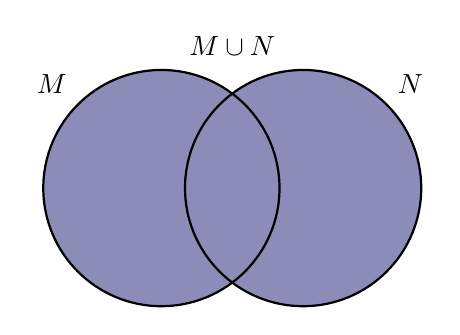
\begin{tikzpicture}[thick,
                set/.style = {circle,
                        minimum size = 3cm,
                        fill=MidnightBlue!50}]
        \node[set,label={135:$M$}] (M) at (0,0) {};
        \node[set,label={45:$N$}] (N) at (1.8,0) {};
        \begin{scope}
                \clip (0,0) circle(1.5cm);
                \clip (1.8,0) circle(1.5cm);
                \fill[MidnightBlue!50](0,0) circle(1.5cm);
        \end{scope}
        \draw (0,0) circle(1.5cm);
        \draw (1.8,0) circle(1.5cm);
        \node at (0.9,1.8) {$M\cup N$};
      \end{tikzpicture}}}$
    }%
    $\vcenter{\hbox{Vereinigungsmenge | Für Mengen M und N: \alert{$M\cup N=\{x: x\in M$ \textbf{oder} $x\in N\}$}}}$
  \end{minipage}
  \onslide<+->
  \begin{minipage}{1\textwidth}
    \centering 
    \scalebox{0.5}{%
      $\vcenter{\hbox{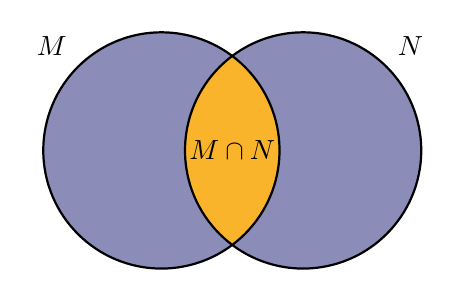
\begin{tikzpicture}[thick,
              set/.style = {circle,
                      minimum size = 3cm,
                      fill=MidnightBlue!50}]
      \node[set,label={135:$M$}] (M) at (0,0) {};
      \node[set,label={45:$N$}] (N) at (1.8,0) {};
      \begin{scope}
              \clip (0,0) circle(1.5cm);
              \clip (1.8,0) circle(1.5cm);
              \fill[Dandelion](0,0) circle(1.5cm);
      \end{scope}
      \draw (0,0) circle(1.5cm);
      \draw (1.8,0) circle(1.5cm);
      \node at (0.9,0) {$M\cap N$};
    \end{tikzpicture}}}$
    }%
    $\vcenter{\hbox{Schnittmenge | Für Mengen M und N: \orongsch{$M\cap N=\{x: x\in M$ \textbf{und} $x\in N\}$}\rule{2.5em}{0em}}}$
  \end{minipage}
  \Halbzeile
  \begin{itemize}[<+->]
    \item Beispiel Vereinigungsmenge
      \begin{itemize}[<+->]
        \item $M=\{\alert<7->{a},\alert<7->{b},\gruen<7->{c}\}$
        \item $N=\{\alert<7->{a},\alert<7->{b},\orongsch<7->{d}\}$
        \item $M\cup N=\{\alert<7->{a},\alert<7->{b},\gruen<7->{c},\orongsch<7->{d}\}$
      \end{itemize}
      \Halbzeile
    \item Beispiel Schnittmenge
      \begin{itemize}[<+->]
        \item $M=\{\gruen<11->{a},\gruen<11->{b},c\}$
        \item $N=\{\gruen<11->{a},\gruen<11->{b}\}$
        \item $M\cap N=\{\gruen<11->{a},\gruen<11->{b}\}$
      \end{itemize}
  \end{itemize}
\end{frame}

\begin{frame}
  {Generalisierte Vereinigungs- und Schnittmenge\only<15>{}}
  \onslide<+->
  \onslide<+->
  \alert{$\bigcup M =\{x: x\in Y$ \textbf{für irgendeine} $Y\in M\}$}\\
  \onslide<+->
  \alert{$\bigcap M =\{x: x\in Y$ \textbf{für jede} $Y\in M\}$}\\
  \Zeile 
  \begin{itemize}[<+->]
    \item Beispiel generalisierte Vereinigungsmenge
      \begin{itemize}[<+->]
        \item $M=\{\{\gruen<7>{a}\},\{\gruen<7>{a},\gruen<8>{b}\},\{\gruen<7>{a},\gruen<8>{b},\gruen<9>{c}\}\}$
        \item $\bigcup M=\{%
            \only<7->{\gruen<7>{a}}%
            \only<8->{,\gruen<8>{b}}%
            \only<9->{,\gruen<9>{c}}%
          \}$
      \end{itemize}
      \Halbzeile
      \onslide<10->
    \item Beispiel generalisierte Schnittmenge
      \begin{itemize}[<+->]
        \item<10-> $M=\{\{\gruen<12>{a}\},\{\gruen<12>{a},\orongsch<13>{b}\},\{\gruen<12>{a},\orongsch<13>{b},\orongsch<14>{c}\}\}$
        \item<11-> $\bigcap M=\{%
            \only<12->{\gruen<12>{a}}
          \}$
      \end{itemize}
  \end{itemize}
\end{frame}

\begin{frame}
  {Differenzmenge und Komplementmenge}
  \onslide<+->
  \onslide<+->
  Differenzmenge | \alert{$M-N=\{x: x\in M$ and $x\not\in N\}$}\\
  \onslide<+->
  Komplementmenge | \alert{$M\backslash N=\{x: x\in N$ and $x\not\in M\}$}\\
  \Halbzeile
  \begin{itemize}[<+->]
    \item Beispiel Differenzmenge
      \begin{itemize}[<+->]
        \item $M=\{\orongsch<7,10>{a},\orongsch<10>{\gruen<7>{b}},\orongsch<10>{\gruen<7>{c}}\}$
        \item $N=\{\orongsch<7>{a}\}$
        \item $M-N=\{\gruen<7>{b},\gruen<7>{c}\}$
      \end{itemize}
      \Halbzeile
    \item Beispiel Komplementmenge
      \begin{itemize}[<+->]
        \item $O=\{\orongsch<10>{a},\orongsch<10>{b},\orongsch<10>{c},\alert<10>{k}\}$
        \item $M\backslash O=\{\alert<10>{k}\}$
      \end{itemize}
      \Halbzeile
    \item Universelles Komplement
      \begin{itemize}[<+->]
        \item die universelle Menge | $U=\{\text{\textit{x: x is an object}}\}$
        \item $\alert{M^{\prime}}=\{x: x\in U\text{ and }x\not\in M\}$
      \end{itemize}
  \end{itemize}
\end{frame}

\begin{frame}
  {Triviale Identitäten}
  \onslide<+->
  \onslide<+->
  \centering 
  \begin{tabular}[h]{lccc}
    Idempotenz      & $M\cup M$         & $=$ & $M$ \\
                    & $M\cap M$         & $=$ & $M$ \\
   Kommutativität   & $M\cup N$         & $=$ & $N\cup M$ \\
                    & $M\cap N$         & $=$ & $N\cap M$ \\
   Assoziativität   & $(M\cup N)\cup O$ & $=$ & $M\cup (N\cup O)$ \\
                    & $(M\cap N)\cap O$ & $=$ & $M\cap (N\cap O)$ \\
   Distributivität  & $M\cup (N\cap O)$ & $=$ & $(M\cup N)\cap (M\cup O)$ \\
  \end{tabular}
\end{frame}

\begin{frame}
  {Interessante Identitäten}
  \onslide<+->
  \onslide<+->
  Komplementgesetze\\
  \Halbzeile
  \begin{itemize}[<+->]
    \item $M\cup\emptyset=M$
    \item $M^{\prime\prime}=M$
    \item $M\cap M^{\prime}=\emptyset$
    \item $X\cap U=U$
  \end{itemize}
  \onslide<+->
  \Zeile
  DeMorgan\\
  \Halbzeile
  \begin{itemize}[<+->]
    \item $(M\cup N)^{\prime}=M^{\prime}\cap X^{\prime}$
    \item DeMorgen begegnet uns in der Logik wieder.
  \end{itemize}
\end{frame}

\section{Funktionen und Relationen}

\begin{frame}
  {Tupel (geordnete Paare, Vektoren)}
  \label{slide:tupel}
  \onslide<+->
  \onslide<+->
  Mengen | \orongsch{ungeordnet} \grau{$\{a,b,c\}=\{a,c,b\}=\{b,a,c\}=\{b,c,a\}=\{c,a,b\}=\{c,b,a\}$}\\
  \Viertelzeile
  \onslide<+->
  Tupel | dasselbe, aber \alert{geordnet} \grau{$\langle a,b\rangle\not=\langle b,a\rangle$}\\
  % <a,b>   = {{a},{a,b}}
  % <a,b,c> = {{a},{a,{{b},{b,c}}}}
  \Halbzeile
  \begin{itemize}[<+->]
    \item tion ohne neues Primitiv | \alert{$\langle a,b\rangle \stackrel{def}{=} \{\{a\},\{a,b\}\}$}
    \item Rekursive Anwendung | \gruen{$\langle a,b,c\rangle=$ ???}
      \Halbzeile
    \item in $\langle a,b\rangle$ | $a$ \alert{erste} und $b$ \alert{zweite Koordinate}
  \end{itemize}
  \Halbzeile
\end{frame}

\begin{frame}
  {Kartesische Produkte \only<30>{}}
  \onslide<+->
  \onslide<+->
  Mengen von Tupeln | $\{<a,b>,<a,c>,<b,c>\}$ usw.\\
  \Viertelzeile
  \onslide<+->
  Kartesisches Produkt | \alert{$S_1\times \cdots \times S_n=\{\langle x_1,x_2,\ldots,x_n\rangle: x_i\in S_i\}$}
  \Halbzeile
  \begin{itemize}[<+->]
    \item Für zwei Mengen | $S_1\times S_2=\{\langle x,y\rangle\|x\in S_1$ and $y\in S_2\}$
      \begin{itemize}[<+->]
        \item $S_1=\{%
            \orongsch<21,24,27>{\gruen<8-10,21-23>{a}},\orongsch<22,25,28>{\gruen<11-13,24-26>{b}},\orongsch<23,26,29>{\gruen<14-16,27-29>{c}}%
        \}$
        \item $S_2=\{%
            \orongsch<8,11,14>{1},\orongsch<9,12,15>{2},\orongsch<10,13,16>{3}%
        \}$
        \item $S_1\times S_2=\{%
            \only<8->{\tuple{\gruen<8>{a},\orongsch<8>{1}}}%
            \only<9->{,\tuple{\gruen<9>{a},\orongsch<9>{2}}}%
            \only<10->{,\tuple{\gruen<10>{a},\orongsch<10>{3}}}%
            \only<11->{,\tuple{\gruen<11>{b},\orongsch<11>{1}}}%
            \only<12->{,\tuple{\gruen<12>{b},\orongsch<12>{2}}}%
            \only<13->{,\tuple{\gruen<13>{b},\orongsch<13>{3}}}%
            \only<14->{,\tuple{\gruen<14>{c},\orongsch<14>{1}}}%
            \only<15->{,\tuple{\gruen<15>{c},\orongsch<15>{2}}}%
            \only<16->{,\tuple{\gruen<16>{c},\orongsch<16>{3}}}%
          \}$
        \item<17-> Achtung | \orongsch{$\tuple{1,a}\not\in S_1\times S_2$ usw.}
      \end{itemize}
      \Halbzeile
    \item<18-> Nomenklatur | $\vec{x}$ für $\langle x_1,x_2,\ldots,x_n\rangle$
      \Halbzeile
    \item<19-> n-faches Produkt | $S^n=\{\vec{s}: s_i\in S$ for $1\leq i\leq n\}$
      \begin{itemize}[<+->]
        \item<20-> $\alert{S_1^2}=\alert{S_1\times S_1}=\{%
            \only<21->{\tuple {\gruen<21>{a},\gruen<21>{a}}}
            \only<22->{,\tuple{\gruen<22>{a},\orongsch<22>{b}}}
            \only<23->{,\tuple{\gruen<23>{a},\orongsch<23>{c}}}
            \only<24->{,\tuple{\gruen<24>{b},\orongsch<24>{a}}}
            \only<25->{,\tuple{\gruen<25>{b},\gruen<25>{b}}}
            \only<26->{,\tuple{\gruen<26>{b},\orongsch<26>{c}}}
            \only<27->{,\tuple{\gruen<27>{c},\orongsch<27>{a}}}
            \only<28->{,\tuple{\gruen<28>{c},\orongsch<28>{b}}}
            \only<29->{,\tuple{\gruen<29>{c},\gruen<29>{c}}}
          \}$ 
      \end{itemize}
  \end{itemize}
\end{frame}

\begin{frame}
  {Relationen}
  \onslide<+->
  \onslide<+->
  \textit{a sieht b}, \textit{a wohnt im selben Stockwerk wie b}, \textit{a macht b Vorwürfe}, \ldots\\
  \Halbzeile
  \begin{itemize}[<+->]
    \item Notationen | \alert{$Rab$, $aRb$, $R(a,b)$, $R(\tuple{a,b})$}
    \item Definitionsmenge (domain) A | \alert{$a\in A$}
    \item Zielmenge, Wertemenge (range) B | \alert{$b\in B$}
    \item Zielmenge = Wertemenge A | \textit{R ist eine Relation in A.}
      \Halbzeile
    \item Relation R = eine \gruen{Menge von Tupeln}
    \item \gruen{$R\subseteq A\times B$}
  \end{itemize}
\end{frame}

\begin{frame}
  {Komplement und Umkehrung}
  \onslide<+->
  \onslide<+->
  Komplement von R | $\alert{R^{\prime}=(A\times B)-R=R\backslash(A\times B)}=\gruen{\{\langle a,b\rangle\ \not\in R\}}$ \gruen{for $R\subseteq A\times B$}\\
  \onslide<+->
  Umkehrung (inverse) von R | \alert{$R^{-1}=\{\langle b,a\rangle:\langle a,b\rangle\in R\}$  for $R\subseteq A\times B$}\\
  \Halbzeile
  \begin{itemize}[<+->]
    \item Beispiel Komplement
      \begin{itemize}[<+->]
        \item $R\stackrel{def}{=}\{\tuple{a,b}: a\text{ ist Lehrer von b}\}$
        \item $\alert{\tuple{\text{Herr Webelhuth, Herr Schäfer}}}\in R$
        \item $R\Prm=\{\tuple{a,b}: a\text{ ist nicht Lehrer von }b\}$
        \item $\orongsch{\tuple{\text{Herr Webelhuth, Frau Klenk}}}\not\in R$,\\
          $\orongsch{\tuple{\text{der Garten meiner Eltern, Frau Klenk}}}\not\in R$ usw.
      \end{itemize}
      \Halbzeile
    \item Beispiel Umkehrung
      \begin{itemize}[<+->]
        \item $R^{-1}=\{\tuple{a,b}:b\text{ ist Lehrer von }a\}$
        \item \grau{$=\{\tuple{a,b}:a\text{ ist Schüler von }\}$}
        \item $\alert{\tuple{\text{Herr Schäfer, Herr Webelhuth}}}\in R^{-1}$
      \end{itemize}
  \end{itemize}
\end{frame}

\begin{frame}
  {Funktionen}
  \onslide<+->
  \onslide<+->
  \textit{a hat Vater b}, \textit{zugelassenes Auto a hat Kennzeichen b}, \textit{b ist der Logarithmus von a}, \ldots\\
  \Halbzeile
  \onslide<+->
  Funktion $f$ | eine Relation, sodass \alert{für jedes $a\in A$ genau ein $\tuple{a,b}\in A\times B$ existiert}\\
  \Zeile
  \begin{itemize}[<+->]
    \item partielle Funktion | Funktion in $A\times B$ sodass\\
      für mindestens ein $a\in A$ kein $\tuple{a,b}\in A\times B$ existiert
    \item \grau{formal meistens | $\bar{f}\subseteq A\times(B\cup\{\bot\})$ mit $\bot$ als \textit{undefiniert}}
  \end{itemize}
\end{frame}

% \frame{\frametitle{Injection, surjection, bijection}
% \begin{itemize}
%   \item<1-> B the range of F, F is \textbf{into} B
%   \item<2-> F from A to B is \textcolor{blue}{\textbf{onto (a \textbf{surjection})} B iff there is no $b_i\in B$ s.t. there is no $\langle a,b_i\rangle\in F$}
%   \item<3-> F from A to B is \textcolor{blue}{\textbf{one-to-one (an \textbf{injection})} iff there are no two pairs s.t. $\langle a_i,b_j\rangle\in F$ and $\langle a_k,b_j\rangle\in F$}
%   \item<4-> one-to-one, onto, and total function: correspondence (bijection)
% \end{itemize}
% }

\begin{frame}
  {Funktionskomposition}
  \onslide<+->
  \onslide<+->
  \textit{b ist die Mutter des Vaters von a} (schwed.\ \textit{farmor}),\\
  \textit{a ist der Kehrwert des Logarithmus von b}, \ldots\\
  \Halbzeile
  \onslide<+->
  Funktionsverknüpfung (composition) | Für $F_1\subseteq A\times B$ und $F_2\subseteq A\times C$: \alert{$F_1\circ F_2\subseteq A\times C$}\\
  \Halbzeile
  \begin{itemize}[<+->]
    \item \alert{farmor | $F=Vater\circ Mutter$} und $\alert{F\subseteq Menschen\times\text{\textit{Frauen}}}$
      \begin{itemize}[<+->]
        \item $\text{\textit{Männer}}=\{Ulrich\ \text{\textit{Schäfer}}, Roland\ \text{\textit{Schäfer}}, Jan\ \text{\textit{Böhmermann}}, \cdots\}$
        \item $Frauen=\{Maria\ \text{\textit{Schäfer}},Frau\ Dr.\ Heide\ \text{Rezepa-Zabel}, \cdots\}$
        \item $Menschen=\text{\textit{Männer}}\cup Frauen$
          \Halbzeile
        \item $\gruen<11->{Vater}\subseteq\{\tuple{\alert<11->{Roland\ \text{\textit{Schäfer}}},\gruen<12->{Ulrich\ \text{\textit{Schäfer}}}},$\\
          $\tuple{Frau\ Dr.\ Heide\ \text{Rezepa-Zabel}, Jan\ \text{\textit{Böhmermann}}}, \cdots\}$
          \Halbzeile
        \item $\orongsch<13->{Mutter}\subseteq\{\tuple{\gruen<14->{Ulrich\ \text{\textit{Schäfer}}},\orongsch<15->{Maria\ \text{\textit{Schäfer}}}},$\\
          $\tuple{Jan\ \text{\textit{Böhmermann}},Frau\ Dr.\ Heide\ \text{Rezepa-Zabel}}, \cdots\}$
          \Halbzeile
        \item $F(\alert<11->{Roland\ \text{\textit{Schäfer}}})=\gruen<11->{Vater}\circ \orongsch<13->{Mutter}(\alert<11->{Roland\ \text{\textit{Schäfer}}})=\orongsch<15->{Maria\ \text{\textit{Schäfer}}}$
      \end{itemize}
  \end{itemize}
\end{frame}

\section{Mehr über Relationen und Mengen}

\begin{frame}
  {Reflexivität}
  \onslide<+->
  \onslide<+->
  Eine Relation R in A ist \ldots\\
  \Zeile
  \centering
  \onslide<+->
  \begin{tabular}{llll}
    \gruen{reflexiv} & gdw & für \textbf{jedes $a\in A$}: $\langle a,a\rangle\in R$ & \textit{ist dasselbe Objekt wie} \\
%              & & & {\scriptsize A: physical objects} \\
    \visible<4->{\orongsch{irreflexiv} & gdw & für \textbf{jedes $a\in A$}: $\langle a,a\rangle\not\in R$ & \textit{ist Vater von} }\\
    \visible<5->{\alert{nichtreflexiv} & gdw & für \textbf{ein $a\in A$}: $\langle a,a\rangle\not\in R$ & \textit{hat gesehen} }\\
  \end{tabular}
\end{frame}

\begin{frame}
  {Symmetrie}
  \onslide<+->
  \onslide<+->
  Eine Relation R in A ist \ldots\\
  \Zeile
  \centering
  \onslide<+->
  \scalebox{0.9}{%
  \begin{tabular}{llll}
                 \gruen{symmetrisch}         & gdw & für jedes $\langle a,b\rangle\in R: \langle b,a\rangle\in R$                         & \textit{hat dasselbe Auto wie} \\
    \visible<4->{\alert{asymmetrisch}        & gdw & für jedes $\langle a,b\rangle\in R: \langle b,a\rangle\not\in R$                     & \textit{hat ein anderes Auto als} }\\
    \visible<5->{\orongsch{nichtsymmetrisch} & gdw & für ein $\langle a,b\rangle\in R: \langle b,a\rangle\not\in R$                       & \textit{ist Mutter von}\visible<7->{\grau{\Up{1}}}}\\
    \visible<6->{\rot{antisymmetrisch}       & gdw & für jedes $\langle a,b\rangle\in R: \tuple{b,a}\not\in R \text{ \textbf{oder} } a=b$ & $\leq$\\}
  \end{tabular}%
  }\\
  \Zeile
  \centering
  \visible<7->{\grau{\footnotesize\Up{1} Wer hat \textit{Dark} gesehen?}}
\end{frame}

\begin{frame}
  {Transitivität}
  \onslide<+->
  \onslide<+->
  Eine Relation R in A ist \ldots\\
  \Zeile
  \centering
  \onslide<+->
  \begin{tabular}{llll}
                 \gruen{transitiv}      & gdw & $\langle a,b\rangle\in R$ and $\langle b,c\rangle\in R:\tuple{a,c}\in R$ & \textit{steht links von} \\
    \visible<4->{\alert{nichttransitiv} & gdw & das Obige stimmt manchmal nicht                         & \textit{mag}}\\
    \visible<5->{\orongsch{intransitiv} & gdw & das Obige stimmt nie                                    & \textit{ist Mutter von}}\\
  \end{tabular}
\end{frame}

\begin{frame}
  {Einordnung}
  \onslide<+->
  \onslide<+->
  Wozu das Ganze?\\
  \Halbzeile
  \begin{itemize}[<+->]
    \item Referenzsemantik und Einteilung der Welt in Mengen
    \item Ausdrücke, die auf Relationen und Funktionen referieren
    \item andere Grundlage: \alert{Logik, denn Sprache=Logik (irgendwie)} 
  \end{itemize}
\end{frame}

\begin{frame}
  {Aufgaben I}
  \onslide<+->
  \begin{enumerate}[<+->]\scriptsize
    \item Sind folgende Mengendefinitionen zulässig?
      \Viertelzeile
      \begin{enumerate}[<+->]\scriptsize
        \item $A=\{a,b,d,e,f,g\}$
        \item $C=\{\text{\textit{x: x ist in keiner Menge enthalten}}\}$
        \item $D=\{\text{\textit{Böhmermann, Horst Lichter}}, \{\}\}$
        \item $E=\{a,b,a,d,e,f,g\}$
        \item $F=\{\text{\textit{r: r ist eine rationale Zahl}}\}\cup\mathbb{N}$
      \end{enumerate}
      \Halbzeile
    \item Sind folgende Aussagen korrekt?
      \Viertelzeile
      \begin{enumerate}[<+->]\scriptsize
        \item $\{\}\subseteq\{blau,rot,gelb\}$
        \item $\{x:x\in A\}=A$
        \item $\{Jan, Horst, Heide\}\not=\{Horst,Jan,Heide\}$
        \item Wenn $A=\{\text{\textit{x:x ist ein Auto}}\}$ und $a\in A$ und außerdem\\
          $B=\{\text{\textit{x:x ist eine Menge von Dingen, die die Umwelt belasten}}\}$ und $A\in B$,\\
          dann folgt daraus $a\in B$.
        \item Wenn $A\subseteq B$ und $B\subseteq A$, dann folgt $A=B$.
        \item Wenn $A\subset B$ und $B\subset A$, dann folgt $A\not=B$.
        \item Wenn $a\in A$ und $a\in B$, dann folgt $a\in A\cup B$.
        \item Wenn $a\in A$ und $a\in B$, dann folgt $a\in A\cap B$.
        \item Wenn $a\not\in A$ und $a\not\in B$, dann folgt $a\in (A\cup B)\Prm$.
      \end{enumerate}
  \end{enumerate}
\end{frame}

\begin{frame}
  {Aufgaben II}
  \begin{enumerate}[<+->]\setcounter{enumi}{2}\scriptsize
    \item Beantworten Sie die folgenden Fragen.
      \Viertelzeile
      \begin{enumerate}[<+->]\scriptsize
        \item Was ist $\wp\{Horst,Heide,Jan\}$?
        \item Beantworten Sie die beiden Fragen auf Folie~\ref{slide:potenzmenge}.
        \item Stimmt es, dass $\{Horst,Heide\}\subset\bigcap\{\{Tschernobyl,Harrisburg\},\{Horst,Heide,Albert\},\{Horst,Webelhuth,Heide,Fukushima\}\}$?
        \item Stimmt es, dass $\{Heide,Harrisburg\}\subseteq\bigcup\{\{Tschernobyl,Harrisburg\},\{Horst,Heide,Albert\},\{Horst,Webelhuth,Heide,Fukushima\}\}$?
        \item Stimmt es für nicht-leere Mengen $A$ und $B$, dass $A\backslash B=B-A$?
        \item Und für leere oder nicht-leere Mengen?
        \item Vervollständigen Sie von Folie~\ref{slide:tupel} \gruen{$\langle a,b,c\rangle=$ ???} (Auflösen von Tupeln in Mengenschreibweise).
        \item Auch wenn es weh tut, dasselbe bitte für $\langle a,b,c,d\rangle$!
        \item Ist Folgendes korrekt: $\tuple{Horst,Heide}=\tuple{Heide,Horst}$?
        \item Ist Folgendes korrekt: $\{\tuple{Horst,Heide},\tuple{Jan,Albert}\}=\{\tuple{Jan,Albert},\tuple{Horst,Heide}\}$?
        \item Was muss der Fall sein, damit $A\circ B=B\circ A$?
        \item Finden Sie ein Beispiel für eine nicht-partielle Funktion von Dingen der realen Welt zu Dingen der realen Welt. Warum ist diese Funktion keine Relation? Finden Sie außerdem ein ähnliches Beispiel für eine partielle Funktion.
        \item Finden Sie je eine Relationen zwischen Dingen der realen Welt, die reflexiv, irreflexiv, nichtreflexiv, symmetrisch, asymmetrisch, nichtsymmetrisch, antisymmetrisch, transitiv, nichttransitiv und intransitiv ist. Die Relationen müssen nicht mit einem bestimmten natürlichsprachlichen Wort ausdrückbar sein (vergleiche viele der Beispiele auf den Folien). In einigen Fällen ist das recht schwierig. Versuchen Sie es ohne Google, ChatGPT usw., sonst bringt es Ihnen nichts.
      \end{enumerate}
  \end{enumerate}
\end{frame}


% \frame{\frametitle{Connectedness}
% A relation  R in $A=\{a,b,\ldots\}$ is...\\
% 
% \bigskip
% {\small
% \begin{tabular}{ll|l}
%   & if & (ex.) \\
%   \hline
%   connected & for every $a,b\in A$, $a\not =b$: & $>$ \\
%             & either $\langle a,b\rangle\in R$ or $\langle b,a\rangle\in R$ & {\scriptsize (A: the natural numbers)} \\
%   non-connected & for some $a,b\in A$  & likes \\
%                 & the above is not the case & \\
% \end{tabular}}
% }

% \frame{\frametitle{Equivalence relations}
% \begin{itemize}
%   \item<1-> reflexive \footnotesize{($\langle a,a\rangle\in R$ for every $a$)}
%   \item<2-> symmetric \footnotesize{($\langle b,a\rangle\in R$ for every $\langle a,b\rangle$)}
%   \item<3-> transitive \footnotesize{($\langle a,b\rangle\in R$ \& $\langle b,c\rangle\in R\rightarrow\langle a,c\rangle\in R$)}
%   \item<4-> \emph{is as stupid as}
%   \item<5-> partition the range into equivalence classes:\\$A=\{a,b,c,d\}$, for example $P_{A_1}=\{\{a,b\},\{c\},\{d\}\}$
%   \item<6-> \textcolor{red}{not} $\{\{a\},\{b,c\}\}$ or $\{\{a,b\},\{b,c\},\{d\}\}$
% \end{itemize}  
% }
% 
% \frame{\frametitle{Defining ordering relations}
% An ordering relation R in A is ...
% \begin{itemize}
%   \item<1-> transitive \footnotesize{($\langle a,b\rangle\in R$ \& $\langle b,c\rangle\in R\rightarrow\langle a,c\rangle\in R$)} \ldots plus \ldots
%   \item<2-> \textcolor{blue}{irreflexive and asymmetric: \textbf{strict order}}
%   \item<3-> {\footnotesize $A=\{a,b,c,d\}$, $R_1=\{\langle a,b\rangle, \langle b,c\rangle, \langle a,c\rangle\}$}
%   \item<4-> \textcolor{blue}{reflexive and anti-symmetric: \textbf{weak order}}
%   \item<5-> {\footnotesize $A=\{a,b,c,d\}$, $R_1=\{\langle a,a\rangle, \langle b,b\rangle, \langle c,c\rangle, \langle a,b\rangle, \langle b,c\rangle, \langle a,c\rangle \}$}  
% \end{itemize}
% }
% 
% \frame{\frametitle{Orders: an example}
% \begin{itemize}
%   \item<1-> a strict order: \emph{greater than} ($>$) in $\mathbb{N}$
%   \item<2-> what is the corresponding weak order
%   \item<3-> $\geq$
% \end{itemize}
% }
% 
% \frame{\frametitle{}
% \begin{itemize}
%   \item<1-> \textbf{minimal}: x is not preceded
%   \item<2-> \textbf{least}: x precedes every other lement
%   \item<3-> \textbf{maximal}: x is not succeeded
%   \item<4-> \textbf{greatest}: x succeeds every other element
%   \item<5-> \textbf{well-ordering}: total order, every subset has a least element
% \end{itemize}
% }

% \section{Mächtigkeiten}
% 
% 
% \frame{\frametitle{The number of elements\ldots}
% \begin{itemize}
%   \item<1-> $A=\{a,b,c\}$
%   \item<2-> $B=\{a,b,c\}$
%   \item<3-> obviously, $A=B$ (equal)
%   \item<4-> there is an $R$ from A to B s.t. $R=\{\langle a,a\rangle,\langle b,b\rangle,\langle c,c\rangle\}$
%   \item<5-> for every set C with the same number of elements\\ (e.g., $C=\{1,2,3\}$): 
%          $R=\{\langle a,1\rangle,\langle b,2\rangle,\langle c,3\rangle\}$
%   \item<6-> such relations are one-to-one correspondences
% \end{itemize}
% }
% 
% \frame{\frametitle{Denumerable sets}
% \begin{itemize}
%   \item<1-> $\mathbb{N}$ is infinite
%   \item<2-> for every A there is some R\Sub{card}
%        \begin{itemize}
%          \item<3-> a one-to-one correspondence
%          \item<4-> from A's members to the first $n$ members of $\mathbb{N}$
%          \item<5-> s.t. $n$ is the \textcolor{blue}{cardinality of A, $\|A\|$}
%       \end{itemize}
%   \item<6-> sets A,B with $\|A\|=\|B\|$ are \textcolor{blue}{equivalent}
%   \item<7-> $\|\mathbb{N}\|=\aleph^0$
% \end{itemize}
% }
% 
% 
% \frame{\frametitle{A problem}
% \begin{itemize}
%   \item<1-> \textcolor{red}{for some sets there is no such R\Sub{card}}
%   \item<2-> no way of bringing their elements into an exhaustive linear order
%   \item<3-> no problem with $\mathbb{Q}$: 
%     \begin{small}\Treek[2]{2}{
% 	    & \K{$\ra{0,1}$}\ARkk{0,0}{0,0}{dl} & \K{$\ra{0,2}$}\ARkk{0,0}{0,0}{dl}\ARr{dll} & \K{$\ra{0,3}$}\ARkk{0,0}{3,0}{dl}\ARr{ddlll} & \K{$\cdots$}\ARkk{0,0}{0,0}{dl}\\
% 	    \K{$\ra{1,0}$} & \K{$\ra{1,1}$}\ARkk{-3,0}{0,0}{dl}        & \K{$\ra{1,2}$}\ARkk{0,0}{0,0}{dl} & \K{$\ra{1,3}$}\ARkk{0,0}{0,0}{dl} & \K{$\cdots$}\ARkk{0,0}{0,0}{dl} \\
% 	    \K{$\ra{2,0}$} & \K{$\ra{2,1}$}\ARkk{0,0}{0,0}{dl}        & \K{$\ra{2,2}$}\ARkk{0,0}{0,0}{dl} & \K{$\ra{2,3}$}\ARkk{0,0}{0,0}{dl} & \K{$\cdots$}\ARkk{0,0}{0,0}{dl} \\
%     \K{$\vdots$}   & \K{$\vdots$}          & \K{$\vdots$}   & \K{$\vdots$}   &  \\
%     }\end{small}
% \end{itemize}
% }
% 
% \frame{\frametitle{The non-denumerable real numbers}
% \begin{itemize}
%   \item<1-> now: $\mathbb{R}$
%   \item<2-> some elements cannot be represented as an ordered pair of two elements of $\mathbb{N}$
%   \item<3-> in $[0,1]$, every real can be represented as \textcolor{blue}{$0.abcdefg\ldots$}, $a,b,c,d,e,f,g,\ldots\in\{0,1,2,3,4,5,6,7,8,9\}$
% \end{itemize}
% }
% 
% \frame{\frametitle{Trying to enumerate}
% \begin{itemize}
%   \item<1-> an enumeration of $[0,1]$ in $\mathbb{R}$?\\
%   
%   \medskip
%   \begin{tabular}{ccccccccc}
%      x\Sub{1} & = & 0 & . & a\Sub{11} & a\Sub{12} & a\Sub{13} & a\Sub{14} & \ldots \\
%      x\Sub{2} & = & 0 & . & a\Sub{21} & a\Sub{22} & a\Sub{23} & a\Sub{24} & \ldots \\
%      x\Sub{3} & = & 0 & . & a\Sub{31} & a\Sub{32} & a\Sub{33} & a\Sub{34} & \ldots \\
%       $\vdots$ & & \vdots &&&&& \\     
%      x\Sub{n} & = & 0 & . & a\Sub{n1} & a\Sub{n2} & a\Sub{n3} & a\Sub{n4} & \ldots \\
%   \end{tabular}
% \end{itemize}
% }
% 
% \frame{\frametitle{Failing to enumerate}
% \begin{itemize}
%   \item<1-> What about an $x_m$ which differs from $x_n$ at $a_{nn}$\\
%   
%   \medskip
%   {\footnotesize\begin{center}\begin{tabular}{ccccccccc}
%      x\Sub{1} & = & 0 & . & \textcolor{red}{a\Sub{11}} & a\Sub{12} & a\Sub{13} & a\Sub{14} & \ldots \\
%      x\Sub{2} & = & 0 & . & a\Sub{21} & \textcolor{red}{a\Sub{22}} & a\Sub{23} & a\Sub{24} & \ldots \\
%      x\Sub{3} & = & 0 & . & a\Sub{31} & a\Sub{32} & \textcolor{red}{a\Sub{33}} & a\Sub{34} & \ldots \\
%       $\vdots$ & & \vdots &&&&& \\     
%      x\Sub{n} & = & 0 & . & a\Sub{n1} & a\Sub{n2} & a\Sub{n3} & \textcolor{red}{a\Sub{nn}} & \ldots \\
%   \end{tabular}\end{center}}
%   
%   \item<2-> \textcolor{red}{It won't be in the array...}
%   \item<3-> $\mathbb{R}$ is non-denumerable
%   \item<4-> If $\|A\|=\aleph^0$ then $\|\wp(A)\|=2^{\aleph_0}$ (cf. Partee et al. 62f.)
% \end{itemize}
% }
